% ICASSP 2027 噪声篇 —— docs/11 计划。数字 \todo 待今晚 H200 数据。
\documentclass{article}
\usepackage{spconfa4}
\usepackage{amsmath,amssymb,amsfonts}
\usepackage{booktabs}
\usepackage{microtype}
\usepackage{url}
\usepackage{graphicx}
\usepackage{xcolor}
\usepackage[hidelinks]{hyperref}
\newcommand{\todo}[1]{\textcolor{red}{[TODO: #1]}}
\newcommand{\lfd}{Lychee-FD}
\newcommand{\vc}{VoiceChat}
\newcommand{\rn}{RN-t}% RNNoise-style torch front-end

\title{Behaviour-Aligned Front-Ends for Full-Duplex Speech LLMs, With and Without Gradients}

\name{Jianming Liu\thanks{Code, recipes and logs: \url{https://github.com/jianmliu/behaviour-aligned-frontends}.}}
\address{Independent Researcher, Newton, USA}

\begin{document}
\maketitle

\begin{abstract}
Hosted full-duplex speech LLMs are absorbing signal clean-up; what remains on the device is a
front-end whose job is to serve the model's \emph{turn-taking decision}---and whose builder may
not own the model. We study how to align a 78\,k-parameter RNNoise-style front-end to that
decision under two regimes: \emph{with} gradients through a frozen open model, and
\emph{without}, from the model's turn decisions alone, as a hosted API would expose. On one open
model (Freeze-Omni) the two are compared directly on the same front-end and objective. As the measurement
instrument we add a controlled noise protocol to the HumDial test set and score first-response
placement. On \lfd\ (12.8\,B), signal-trained suppression restores audibility and with it every
clean-condition pathology, while behaviour-level training cuts wrong-place responses from
67\,\% to 48\,\% ($p<10^{-23}$, paired) at no cost in on-time responses: signal restoration is
not behaviour restoration. On Freeze-Omni (7B) we train an event-level placement objective with
gradients and by evolution strategies on decisions only. This eager model's failures are linguistic and a waveform front-end has no leverage at moderate noise; once masking is severe enough ($-$15\,dB) to make noise a trigger, gradient alignment reverses the front-end's effect (later take-overs, $p<10^{-35}$ vs.\ the frozen suppressor) while a 23-dimensional black-box policy with 3k rollouts stays at the signal solution: at the budgets tried, the price of losing gradients is the whole effect. Protocol,
metrics and recipes are released.
\end{abstract}
\begin{keywords}
full-duplex speech LLM, noise suppression, turn-taking, false barge-in, behaviour-aware front-end
\end{keywords}

\section{Introduction}
\label{sec:intro}
% 段1: 全双工模型与行为暴露面
Full-duplex spoken dialogue models emit agent audio while ingesting user audio, so their core
competence is a continuous decision: speak, keep listening, or back-channel. That decision is made
from raw acoustics. For transcription-oriented pipelines, decades of work hardened recognition
against noise; the \emph{turn-taking} decision of a full-duplex model has no such history, and it
fails differently---not by mis-hearing words but by \emph{acting}: answering a slammed door,
treating caf\'e babble as a barge-in.

% 段2: 证据与基准空白（HumDial 自证）
The evidence is already on the record. The ICASSP HumDial challenge~\cite{humdial2026}, whose
dual-channel benchmark is the most recent standard for full-duplex interaction, reports that
across submitted systems ``robustness under background noise remains limited, with transient
noises causing false activations or missed detections''---and yet the benchmark itself, like
Full-Duplex-Bench and its successors~\cite{lin2025fdb,lin2025fdb15,fdbv3}, contains no noise
condition. The gap reaches the commercial frontier: OpenAI's GPT-Live-1, released to its API
this month, is full-duplex, removes the separate turn detector from the audio path, reports a
30-point gain on Full-Duplex-Bench, and claims ``improved handling of ambient noise''---without a
single noise-condition number~\cite{gptlive2026}. The community has named the failure and does
not yet measure it.

% 段3: 部署答案=前端;前端训练目标错位;托管时代新前端的规格
The deployed answer to noise is an upstream suppressor---in the open-source stack, most commonly
RNNoise~\cite{valin2018rnnoise} and its descendants, built and tuned against signal metrics on
data the downstream model never sees. Hosted full-duplex models change what such a front-end is
\emph{for}. Signal clean-up is being absorbed into the model; what stays on the device is what
the cloud cannot do: decide, cheaply and privately, whether a sound is addressed to the system
and whether a turn is coming---before a metered session sees it. A front-end with that job must
be aligned to the \emph{behaviour} of a model its builder may not own and cannot backpropagate
through. Whether signal-metric training serves the turn-taking decision, and whether
behaviour-level alignment is reachable with and without gradients, are the questions this paper
measures, with the model held frozen throughout.

% 段4: 为什么行为目标这次能成（无反馈环）
A companion line of work on \emph{acoustic echo} found that even cross-entropy on the model's own turn-taking tokens leaves an objective--behaviour gap dominated by teacher-forcing \emph{exposure}: echo is the model's own output fed back, and the states that break the benchmark are never visited under teacher forcing (companion work, in submission). Noise carries no such loop---it is exogenous, ``do not activate on this'' is an ordinary conditional decision fully covered by teacher-forced supervision, and 78\,k parameters leave little room for degenerate shortcuts. If behaviour-level training of a front-end works anywhere, it should work here.

% 段5: 贡献
Contributions. (1)~\emph{Two regimes, one testbed} (Freeze-Omni, 7B): we align the same 78\,k front-end to the
same frozen model under the same placement objective (a)~with gradients through the model and
(b)~without---by evolution strategies on the model's turn decisions alone, the interface a hosted
API exposes. Neither has leverage at moderate noise; where severe masking creates an acoustic failure, (a) reverses the front-end's effect and (b) does not at any budget tried, even given (a)'s own loss as reward---the measured price of losing gradients. (2)~The measurement instrument: a
noise-augmented behavioural protocol on the HumDial test set scoring first-response
\emph{placement}, grounded in the benchmark's respond/refrain semantics (\S\ref{sec:protocol}).
(3)~With gradients on \lfd: signal-trained suppression restores audibility and with it every
clean-condition pathology, while behaviour-level training cuts the wrong-place total from 67 to 48\,\%
($p<10^{-23}$, paired) at no cost in on-time responses---signal restoration and behaviour
restoration come apart (\S\ref{sec:results}). (4)~Released protocol, metrics, recipes and logs.

\section{Setup}
\label{sec:protocol}
\subsection{Model and behaviour semantics}
\lfd~\cite{lychee2026fd} (12.8\,B) emits explicit turn-taking \emph{control tokens} every
0.4\,s chunk (\texttt{keep-listening}, \texttt{start-speaking}, backchannel, \ldots): its
behaviour is directly observable and directly supervisable. Audio enters as continuous encoder
features, so gradients pass through the frozen model into a front-end.

\subsection{Noise protocol on HumDial}
The HumDial English test set groups 4{,}550 recordings into ten scenarios with explicit
respond/refrain semantics: four demand a response (\texttt{ask}, \texttt{repeat}, \texttt{shift},
\texttt{deny}); six demand restraint (\texttt{backchannel}, \texttt{wait}, \texttt{pause},
\texttt{talk\_to\_others}, two \texttt{others\_talk\_to\_user} variants). We take
100/scenario, add noise from held-out DEMAND environments at SNR
$\in[0,15]$\,dB (per-sample seeded: all systems see bit-identical scenes), and feed
the frozen model offline. Offline decoding of these long, two-turn recordings yields, in practice, a single model
response per sample (99\,\% of clean decodes), so we measure the \emph{placement} of that
response---a quantity with clean semantics per scenario and direct sensitivity to noise:
\textbf{on-time} (at or after the end of the user's question), \textbf{premature} (inside the
question---a failure HumDial itself reports for current models on slow speech), \textbf{miss}
(no response), \textbf{mis-addressed} (placed inside speech directed at someone other than the
model: the third-party segments of the \texttt{others\_*} and \texttt{talk\_to\_others}
scenarios---the direct false-trigger read-out), and \textbf{break-preempt} (inside an annotated
mid-question pause). Clean decoding (L0) anchors the distribution; the noise effect is the
\emph{paired shift} of this distribution on bit-identical samples, which is robust to the
imperfect clean baseline. That baseline is imperfect by design, not by accident: premature
take-overs dominate it for both models, which is the behaviour HumDial's organisers report
for current systems on slow or paused speech, and offline decoding of a two-turn recording
exposes it fully because nothing interrupts the model once it starts. The metric therefore
measures the placement of a decision the models really make, and every comparison in this
paper is a within-sample contrast against that same baseline.

\subsection{Front-end and training ladder}
\rn\ is a differentiable RNNoise-style suppressor: 22 Bark-band features, the original
Dense--GRU--GRU--GRU--Dense gain topology (78\,k parameters), band gains interpolated to STFT
bins, length-preserving. Signal-loss pretraining (SI-SNR, speech from a disjoint corpus, DEMAND
ch01) reaches +9.3\,dB held-out gain at SNR~5 with 32.5\,dB clean-speech fidelity.
\textbf{R-indep} freezes this checkpoint---deployment practice. \textbf{R-joint} fine-tunes it
through the frozen model against cross-entropy on the model's own clean-run control-token
trajectory (self-distillation; the released transition-preserving label subsampling), on a
training corpus disjoint from HumDial (Full-Duplex-Bench~1.0 user audio, 429 recordings
$\le$20\,s, DEMAND noise re-drawn per step). The comparison
isolates exactly one variable: what the training objective knows about the model being served.

\section{Results}
\label{sec:results}

\begin{figure}[t]
\centering
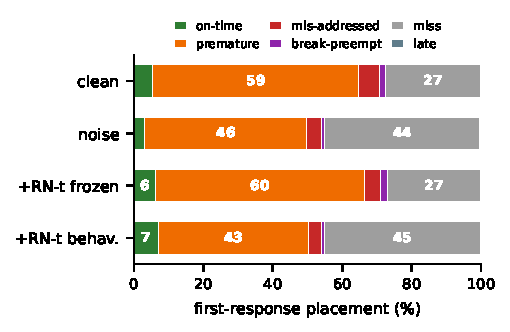
\includegraphics[width=\columnwidth]{fig_placement.pdf}
\caption{First-response placement across the four conditions (1000 paired samples). Noise
collapses responses into misses; the frozen suppressor restores the clean profile, pathologies
included; the behaviour-fine-tuned one shrinks every wrong-place class instead.}
\label{fig:placement}
\end{figure}

\begin{table}[t]
\centering
\caption{First-response placement on the HumDial test set (1000 samples, 100/scenario;
identical noise per sample across all noisy conditions). Mis-addr.\ = response placed inside
third-party speech (false trigger); break-pre.\ = response inside an annotated mid-question
pause (\% of the \texttt{pause} scenario). \rn-frozen = signal-pretrained, frozen (R-indep);
\rn-behav.\ = same start, fine-tuned on control-token CE (R-joint).}
\label{tab:main}
\begin{tabular}{lcccc}
\toprule
\% & clean & noise & +\rn-frozen & +\rn-behav. \\
\midrule
on-time $\uparrow$      & 5.4  & 3.2  & 6.2  & \textbf{7.0} \\
premature $\downarrow$  & 59.4 & 46.4 & 60.1 & \textbf{43.3} \\
miss $\downarrow$       & 27.4 & 44.5 & \textbf{26.6} & 44.7 \\
mis-addr.\ $\downarrow$ & 5.8  & 4.4  & 4.8  & \textbf{3.7} \\
break-pre.\ $\downarrow$& 18   & 10   & 20   & \textbf{10} \\
\bottomrule
\end{tabular}
\end{table}

\subsection{Noise breaks the turn-taking decision}
Table~\ref{tab:main}, first two columns. The clean baseline already carries the pathologies
HumDial reports for current systems---premature answers dominate (59.4\,\%; 86\,\% on
\texttt{talk\_to\_others}), and 58\,\% of \texttt{others\_talk\_to\_user\_before} decodes fire
inside speech addressed to a third party. Noise does not add new misbehaviour on top; it
\emph{deafens}: misses rise in all ten scenarios (worst on \texttt{repeat}, $42\to59$), on-time
responses halve, and every hearing-dependent failure---premature, mis-addressed, pause
preemption---falls passively with the signal. The same direction reproduces on \vc-11B under our companion echo protocol's noise-only
control (self-talk $1.60\to1.94$, premature take-overs $1.09\to1.39$ events/min).

\subsection{Frozen versus behaviour-fine-tuned suppression}
Table~\ref{tab:main}, last two columns, one training variable apart. The frozen suppressor is a
faithful restorer: misses return to the clean level (26.6\,\%) and so does everything
else---premature back to 60.1\,\%, pause preemption at 20\,\%, false triggers at 4.8\,\%. Signal
fidelity hands the model back its clean-condition behaviour, pathologies included.
The behaviour-fine-tuned front-end spends the same capacity differently: 17\,pt fewer premature
answers than the frozen variant (paired exact McNemar on bit-identical samples: 86 vs 252
discordant pairs, $p=5{\times}10^{-20}$), the lowest false-trigger rate of any condition
(3.7\,\%), and half the pause preemptions---while misses stay at the noise level (44.7\,\%,
$p=2{\times}10^{-22}$). Aggregating the three wrong-place classes
(premature\,+\,mis-addressed\,+\,break-preempt) gives 66.9\,\% for the frozen front-end against
48.0\,\% for the behaviour-trained one ($p=4{\times}10^{-24}$), at no measurable cost in
correct responses: on-time is 7.0\,\% against the frozen variant's 6.2\,\% and the clean
baseline's 5.4\,\% (both n.s.). The trade it learns is legible: speak when the decision evidence
survives the noise, stay silent when it does not, rather than reconstruct everything the model
might react to.

\subsection{Second model: with and without gradients}
\label{sec:fo}
A hosted model exposes no logits and no gradients---only its behaviour. To test whether
behaviour-level alignment survives that interface, we repeat the protocol on
Freeze-Omni~\cite{freezeomni2024} (7B, frozen Qwen2 backbone, a chunk-level \emph{state head}
that decides when to speak; listening needs no token generation, so placement is read from that
decision alone) on the same 1{,}000-sample protocol (200 samples, 20/scenario, for the ES and
self-distillation variants and the clean-audio and probe rows), and train the same 78\,k
front-end two ways from the same signal-pretrained start: (a)~a differentiable \emph{expected placement cost}
(first-trigger distribution over chunks $\times$ premature/on-time/miss costs, refrain samples
penalising any trigger, plus a logit-margin term in the premature region so that a saturated
decision still carries gradient) with gradients through the frozen model; (b)~evolution strategies on the
realised placement reward, using nothing but the model's turn decisions. Freeze-Omni's clean
profile is the mirror image of \lfd's: on-time 40.6\,\%, premature 43.8\,\%, no misses---and no
restraint: it fires inside third-party speech in 99/100 \texttt{others\_before} samples and
inside the pause gap in 57/100. Noise at the protocol's SNR (0--15\,dB) does not move it at
all (on-time 40.6\,\%, premature 43.4\,\%, restraint axes 100/100 and 60/100): an eager model
is not deafened. Pushed further, an acoustic share does appear---but as \emph{more} eagerness,
not silence: at $-$5, $-$10, $-$15 and $-$20\,dB premature take-overs rise to 46.3, 51.2, 56.5 and 63.0\,\%
(1{,}000 samples each) with still no misses; sustained masking acts as a trigger, whereas three 300\,ms bursts at +10/+20\,dB barely register (42.5/40.0, 39.5/43.5): HumDial's transient false activations are not this model's failure mode. Two
consequences follow. Self-distillation cannot be the target here---on Full-Duplex-Bench the
model's own clean first response precedes the annotated end of the user's turn by a median
7.3\,s (90\,\% of samples $>$1\,s early)---so we take the benchmark's turn-end annotations as
placement targets; and the front-end's job is restraint rather than restoration, so we also check clean audio,
where all three front-ends leave placement unchanged (200 samples, n.s.). Under noise, the frozen suppressor nudges
the model slightly \emph{more} eager (on-time 38.8\,\%, premature 45.1\,\%, restraint axes
100/100 and 61/100: cleaner speech, if anything earlier take-over). The behaviour-trained
front-ends land on the noisy baseline---soft placement with
annotation targets 39.7/44.3 on 1{,}000 samples, restraint axes 100/100 and 60/100 exactly as
without it; on 200 samples, self-distillation targets 43.0/39.0 and ES 37.5/45.5
(on-time/premature), all within sampling noise. Per sample, noise moves 32\,\% of decision instants symmetrically; the front-ends move 25--29\,\%, and the \emph{wrong} way for restraint---earlier take-overs outnumber later ones 172:115 (frozen) and 156:91 (trained), sign test $p<10^{-3}$: cleaner speech makes an eager model marginally more eager. The trained suppressor kept 6.4 of the frozen model's 8.6\,dB SI-SNR gain on its training mixtures: nothing
collapsed, and the only direction found was the acoustic one. \emph{Where the acoustic share exists, the leverage appears.} At $-$15\,dB (1{,}000 paired
samples; 28.4/56.5 without a front-end) the frozen suppressor makes matters worse---24.3/61.2, decisions earlier 340:174 (sign test $p=2{\times}10^{-13}$): denoising feeds the trigger. The behaviour-trained front-end moves them the other way: 35.8/49.0, later 309:173 against no front-end ($p=6{\times}10^{-10}$) and 432:139 against the frozen suppressor ($p<10^{-35}$). The same 78\,k parameters, aligned to the decision
instead of the signal, reverse the front-end's effect: the \lfd\ finding on a second model. The black-box arm does not follow: evolution strategies over a 23-parameter band-gain policy (40 generations, 3k rollouts) end at 24.7/60.8, indistinguishable from the frozen suppressor ($p=0.27$) and earlier than the gradient-trained front-end 421:154. All 78\,k parameters at the same budget only wander (17.4/68.7, $p<10^{-11}$ vs.\ frozen). Tripling the generations (120) barely moves it (24.6/60.5), and the gradient arm's own dense loss as reward does not help either (25.9/59.5; 23.6/61.5 over all 78\,k parameters): the price is the direction, not the reward or the budget. At $-$10\,dB the pattern replicates: frozen earlier (28.8/55.7 vs.\ 32.9/51.2; 294:168), gradient-aligned later (36.9/47.1; 356:150 vs.\ frozen), black-box at or past the frozen solution (27.1/57.6; 392:145 earlier than gradient-aligned), all $p<10^{-8}$. At $-$5\,dB the frozen suppressor still harms (32.4/51.9 vs.\ 37.7/46.3); gradient alignment only cancels that harm (38.2/46.1). Content follows: judged by Qwen2-7B-Instruct on the opening of the first response (0--2 relevance, $-$15\,dB), the frozen suppressor lowers relevance (0.77 vs.\ 0.83, $p=0.07$), gradient alignment keeps it (0.84; 170:132 above frozen, $p=0.03$) and cuts hallucinated Chinese openings from 13.6 to 9.4\,\% ($p=2{\times}10^{-4}$): later take-overs cost no relevance. Across regimes, a waveform front-end has leverage only over the acoustic share of a
failure---large on \lfd, near zero here.

\subsection{Ablations: two attractors, no middle ground}
\label{sec:abl}
Three variants probe what the behaviour objective needs. (i)~\emph{Gentler learning rate}
($3{\times}10^{-5}$ vs $10^{-4}$): the fine-tune never leaves the pretrained signal
solution---its profile is indistinguishable from the frozen front-end (on-time 6.2\,\%,
premature 62\,\%, miss 25\,\%). (ii)~\emph{Scratch start}: without signal pretraining the same
objective learns nothing usable; the profile matches raw noise (on-time 3.6\,\% vs 3.2\,\%).
(iii)~\emph{SI-SNR anchor} added to the CE ($\lambda{=}0.05$): the anchor dominates and the
solution reverts to the frozen profile, restraint gains included. The picture is consistent:
the signal solution and the behaviour solution are distinct attractors---behaviour training
must start from signal competence (ii), needs enough learning rate to escape it (i), and is
not reachable as a regularised compromise (iii). The objective is not a seasoning over signal
fidelity; it selects a different front-end.

\section{Discussion}
\label{sec:discussion}
\textbf{Where front-ends still pay.} Egocentric-device challenges chart the decline of the generic front-end: in CHiME-8 MMCSG~\cite{zmolikova2024mmcsg} training data beat array processing on WER, yet a neural separation front-end won the \emph{speaker-attribution} axis~\cite{pang2024seuee}; by SLT 2026 SmartGlasses~\cite{smartglasses2026} the winner used no front-end at all. The opposite reaction grows the front-end into a 30B LLM trained on task labels (UAF~\cite{uaf2026}). Our results locate the surviving value: a front-end pays on the axis its objective shares with the downstream decision---attribution there, turn-taking here---and 78\,k parameters aligned to that decision shift behaviour where signal restoration does not. Deployment follows: with
hosted full-duplex models metered per minute of audio, every
noise-induced wrong-place response is a billed event, and an on-device front-end that removes
them at zero marginal cost is a cost control, not an audio-quality option. The same
judgement---is this addressed to the system, is a turn coming---is what an on-device gate needs
to decide when a metered session should be open at all; we leave that gate to future work. Unlike
enhancement-for-ASR joint training, the model is frozen, the target is behaviour rather than
transcription, and the failure repaired (acting at the wrong time) has no transcription analogue.

\textbf{Relation to the echo domain.} In the companion echo setting the same CE failed to move free-running behaviour because teacher forcing never visits the states echo creates; here the perturbation is exogenous and the same objective moves behaviour---consistent with the exposure account. What remains is an \emph{objective} gap: the CE optimum under noise is a restraint profile, reachable only from a signal-competent start (\S\ref{sec:abl}).

\textbf{Limitations.} English subset only; offline decoding of the official test set (no
streaming latency axis); front-ends trained through two models (the \vc\ corroboration is
measurement-only); single noise corpus (DEMAND), though held out between pretraining and test; one LLM judge, opening sentences only; the black-box arm is run on Freeze-Omni only.

\section{Conclusion}
We measured what noise does to the turn-taking decision of a frozen full-duplex speech LLM on
the benchmark that first named the problem, and compared the deployed remedy---a
signal-trained suppressor---against the same suppressor fine-tuned on the model's own
turn-taking tokens. Signal training restores what the model hears; behaviour training changes
what the model does: the wrong-place total falls from 67 to 48\,\% ($p<10^{-23}$, paired), on-time
responses are preserved, and the cost is silence where the evidence does not survive the noise.
The two solutions are separate attractors, not ends of a dial. On a second, eager model the same
alignment reverses the frozen suppressor's effect once masking creates an acoustic failure;
decision-only search does not find that direction. This reframes the front-end
question for deployment: the choice is not how much to denoise, but which decision the
denoiser should serve.

\textbf{Use of AI.} Language-model assistants (Anthropic Claude) drafted and refactored code, ran and monitored the experiment queues, and edited prose; every experiment, number and claim was checked by the author, who takes full responsibility for them.

\clearpage
\bibliographystyle{IEEEbib}
\bibliography{refs}
\end{document}
